\subsection{Propiedades topol\'ogicas de los conjuntos convexos}

A continuaci\'on desarrollaremos algunas propiedades topol\'ogicas para conjuntos convexos \cite{no-lineal}. Como 
un preliminar a esta parte tendremos que dado un punto $x \in \mathbb{R}^n$ un 
$\varepsilon$-vecindario alrededor del conjunto es $N_{\varepsilon}(x)= \{y: \parallel y - x \parallel < \varepsilon\}$.
Primero revisaremps las definiciones de: clausura, interior y frontera de un conjunto arbitrario en $\mathbb{R}^n$,
usando el concepto de $\varepsilon-$vecindario.\\

{\definicion: Sea $S$ un conjunto arbitrario en $\mathbb{R}^n$. 
\begin{itemize}
   \item {\bf Clausura}: Se dice que un punto $x \in \mathbb{R}^n$ est\'a en la clausura de $S$ si \linebreak
	 $\forall \, \varepsilon > 0, \,\,\,\,S\cap N_{\varepsilon}(x) \neq \emptyset $
   \item {\bf Interior}:Un punto $x$ se dice que est\'a en el interior de $S$ si \linebreak
	 $\exists \varepsilon > 0$\, tal que $N_{\varepsilon}(x) \subset S$.
   \item {\bf Frontera}: Un punto $x$ se dice que est\'a en la frontera si $\forall \, \varepsilon > 0$ se tienen que \linebreak
	 $N_{\varepsilon}(x) \cap S \neq \emptyset\,$ y $\,N_{\varepsilon}(x) \cap S^{c} \neq \emptyset$
   \item {\bf Acumulaci\'on}: Un punto $x$ es de acumulaci\'on de $S$ si \linebreak
	 $\forall \,\, \varepsilon > 0$ se tiene que $(N_{\varepsilon}(x)-\{x\}) \cap S \neq \emptyset$
\end{itemize}
\label{top-notable}}

\medskip

\textbf{Notaci\'on:}
\begin{itemize}
   \item Denotaremos por $\, \overline{S}$ a la clausura del conjunto $S$. Adem\'as se tiene que $S$ es cerrado si $\overline{S} = S$.
   \item Denotaremos por $\, \mathring{S}$ al interior del conjunto $S$ y \'este es abierto cuando $\mathring{S}=S$
   \item Denotaremos por $\,fr(S)$ a la frontera del conjunto $S$.
   \item Denotaremos por $\, S'$ al conjunto de puntos de acumulaci\'on de $S$
\end{itemize}

\medskip

Finalmente, un conjunto es acotado si puede ser contenido en una bola bola de radio suficientemente grande. Un conjunto es 
{\itshape compacto} si es cerrado y acotado. Note que el complememeto de un conjunto abierto en un conjunto cerrado (viceversa)
y que los puntos de acumulaci\'on de cualquier conjunto y su complemento son el mismo.\\

\medskip

una manera un poco m\'as f\'acil de asimilar \'estas definiciones es de forma gr\'afica considerando
$S = \{(x, y): x^2 + y^2 \leqslant 1\}$, este conjunto representa todos los puntos dentro del circulo con centro $C(0, 0)$ y 
radio $r=1$. (V\'ease \ref{top})\\

F\'acilmente se puede verificar que $S$ es cerrado, es decir, $\overline{S} = S$.\\
Adem\'as $\mathring{S}$ consiste en todos los puntos que est\'an estrictamente dentro del circulo, esto es,
$\mathring{S} = \{(x, y): x^2 + y^2 < 1 \}$.\\
Finalmente, $S'$ consiste de los puntos en el circulo, esto es, $S' = \{(x, y): x^2 + y^2 = 1\}$.

%------------------------------------topologia de un conjunto--------------------------------------------------------------------
\begin{figure}[h]
  \centering
  \subfigure[Cerradura $\overline{S}$]{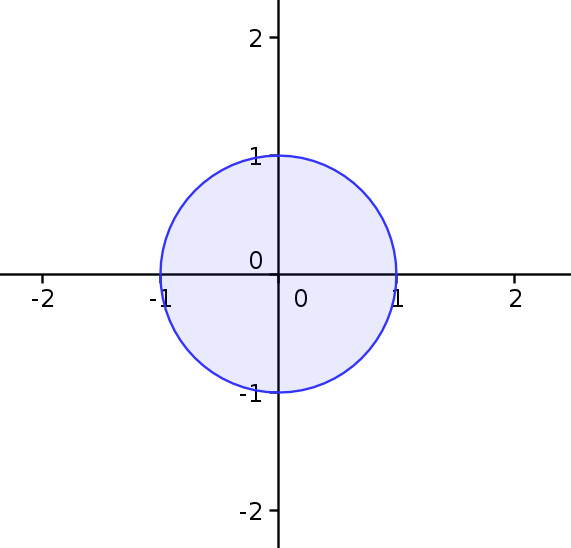
\includegraphics[scale = 1]{./partes/sub_sec/topo.jpg}}
  \subfigure[Interior $\mathring{S}$]{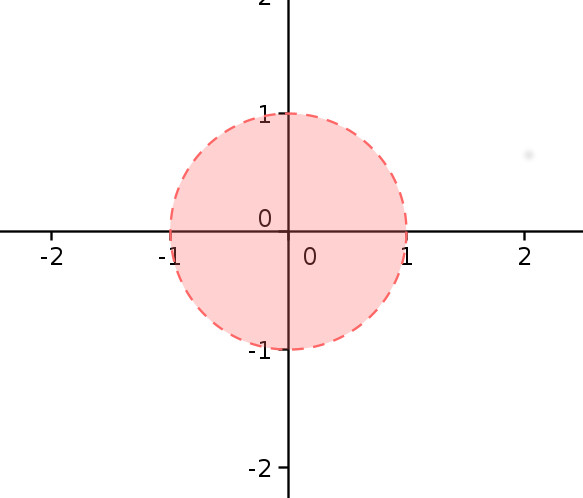
\includegraphics[scale = 1]{./partes/sub_sec/topo_cl.jpg}}
  \subfigure[Acumulaci\'on $S'$]{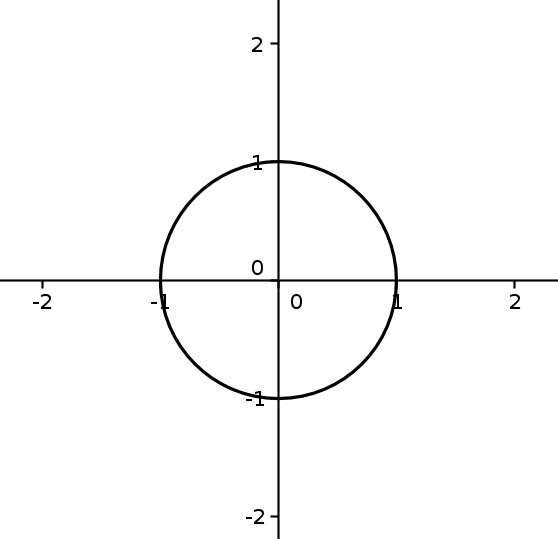
\includegraphics[scale = 1]{./partes/sub_sec/topo_ac.jpg}}
  \caption{Topolog\'ia del conjunto $S = \{(x, y): x^2 + y^2 \leqslant 1\}$}
\end{figure}\label{top}

%---------------------------------------------------------------------------------------------------------------------------------

~\\ \\

\textbf{Caracterizaciones de conjuntos}\\

\begin{itemize}%verificar que item 3 sea abierto
   \item Un conjunto $S$ es cerrado si y solo si contiene todos sus puntos de acumualci\'on, es decir $S' \subset S$.
   \item $\overline{S} = S \cup S'$ es el cerrado m\'as peque\~no que contiene al conjunto $S$.
   \item Un conjunto $S$ es abierto si y solo si \'este no contiene ninguno de sus puntos frontera, mas precisamente $S' \cap S = \emptyset$.
   \item $\mathring{S} \subseteq S$, por la tanto, tenemos que $\mathring{S} = S - S'$ mientras que necesariamente
	$S' \neq S - \mathring{S}$.
\end{itemize}

Un conjunto puede ser ni abierto ni cerrado, los \'unicos conjuntos que son abiertos y cerrados a la vez son el conjunto vac\'io
($\emptyset$) y el mismo $\mathbb{R}^n$. Tambi\'en consideremos que ning\'un punto $\overline{x} \in S$ puede ser un punto interior o de 
acumulaci\'on de $S$. Sin embargo $S \neq \mathring{S} \cup S'$, es decir que $S$ no necesita contener sus puntos de acumulaci\'on.\\ 

Existe otra definici\'on equivalente de conjunto cerrado, el cual es muy importante demostrando desde el punto de vista que es un
conjunto cerrado.\\Esta definici\'on est\'a basada en las sucesiones de puntos contenidos en $S$. \\
Un conjunto es cerrado si y solo si para cualquier sucesi\'on convergente de puntos $\{ x_k \} _{k \in \mathbb{N}} \in S$ con punto
l\'imite $\overline{x}$, as\'i mismo tenemos que $\overline{x} \in S$.\\
La equivalencia de \'esta y la definici\'on previa de cerradura es f\'acilmente de ver ya que el punto l\'imite $\overline{x}$ de 
cualquier sucesi\'on convergente de puntos en $S$ debe encontrarse en el interior o de acumulaci\'on de $S$, en otras palabras
deber\'ia existir un $\varepsilon > 0$ tal que $\{x: \parallel x - \overline{x} \parallel < 0 \} \cap S = \emptyset$ contradiciendo
que $\overline{x}$ es el punto l\'imite de una sucesi\'on contenida en $S$.\\

%llevar un mejor orden en la parte topolog\'ia y ya aplicado a conjuntos convexos y esta otra

\textbf{Segmento de linea entre puntos del interior y cerradura de un conjunto \cite{no-lineal}}\\

Dado un conjunto convexo con interior no vac\'io, el segmento de linea (excluyendo los puntos finales) que une un punto del interior
del conjunto con un punto de la clausura de este pertenece al interior del conjunto. Este resultado se muestra acontinuaci\'on.\\


{\teorema Sea $S$ un conjunto convexo en $\mathbb{R}^n$ con interior no vac\'io. Sea $x_1 \in \overline{S}\,$ y $\, x_2 \mathring{S}$.
Entonces $\lambda x_1 + (1 - \lambda)x_2 \in \mathring{S}~\,\,\, \forall \,\,\,\, \lambda \in (0, 1)$ \label{t_int}}\\

\textbf{\itshape Demostraci\'on: }\\
Como $x_2 \in \mathring{S}\,$ existe un $\varepsilon > 0$ tal que $\{z: \parallel z - x_2 \parallel < \varepsilon\} \in S$. Sea $y$ tal que

\begin{equation}
   y = \lambda x_1 + (1 - \lambda)x_2;~ \lambda \in (0, 1)
   \label{convx}
\end{equation}


Para probar que $y \in \mathring{S}$ es suficiente construir un vecindario sobre $y$ que tambi\'en pertenece a $S$. En particular 
mostraremos que $\{z: \parallel z - y \parallel < (1 - \lambda)\varepsilon\}.$ Sea $z$ tal que 
$\parallel z - y \parallel < (1 - \lambda)\varepsilon$ (v\'ease \ref{convx}), ahora bien, como $x_1 \in \overline{S}$

\[\left \{x: \parallel x - x_1 \parallel < \dfrac{(1 - \lambda)\varepsilon - \parallel z - y \parallel}{\lambda} \right \} \cap S\]

es no vac\'io, en particular, existe $z_1 \in S$ tal que 

\begin{equation}
   \parallel z_1 - x_1 \parallel < \displaystyle{\dfrac{(1 - \lambda)\varepsilon - \parallel z - y \parallel}{\lambda}} 
   \label{casi}
\end{equation}


Ahora, sea $z_2 = \dfrac{z - \lambda z_1}{1 - \lambda}$ de (\ref{convx}), la desigualdad de Schwartz y (\ref{casi}) tenemos: 

\begin{eqnarray*}
   \parallel z_2 - x_2 \parallel = \parallel \dfrac{z - \lambda z_1}{1 - \lambda} - x_2 \parallel &=& \displaystyle{\parallel \dfrac{(z - \lambda z_1) - (y - \lambda x_1)}{1 - \lambda} \parallel} \\  
   &=& \dfrac{1}{1 - \lambda} \displaystyle{ \left\| (z - y) + (x_1 - \lambda x_1) \right\|} \\
  & \leqslant & \dfrac{1}{1 - \lambda} (\parallel z - y \parallel + \lambda \parallel x_1 - z_1 \parallel)\\
  &<& \varepsilon
\end{eqnarray*}

Por lo tanto, $z_2 \in S.$ Dada la definici\'on de $z_2$ notemos que  $z = \lambda z_1 + (1 - \lambda)z_2$, como $z_1\,$ y $\, z_2$
pertenecen a $S$, entonces $z$ tambi\'en pertenece a $S$. Hemos mostrado que para cualquier $z$ con $\parallel z - y \parallel < 
(1 - \lambda)\varepsilon$ pertenece a $S$. Por lo tanto $y \in \mathring{S}. \\$ 
\begin{flushright}
  $\square$ 
\end{flushright}


{\corolario Sea $S$ un cojunto convexo. Entonces $\mathring{S}$ es convexo. \label{int-convx}}

{\corolario Sea $S$ un conjunto convexo con interior no vac\'io. Entonces $\overline{S}$ es convexa. \label{cl-convx}}\\

\textbf{\itshape Demostraci\'on}\\
Asumiendo que $\mathring{S} \neq \emptyset$. Sea $x_1, x_2 \in \overline{S}$, por teorema tenemos que 
$$\lambda x_2 + (1 - \lambda)z \in \mathring{S}\,\,\,\, \forall \,\,\lambda \in (0, 1)$$

Sea $\mu \in (0, 1)\,$ fijo. Por teorema \ref{t_int}:
$$\mu x_1 + (1 - \mu)[\lambda x_2 + (1 - \lambda)z] \in \mathring{S} \subset S \,\,\,\, \forall \, \lambda \in (0, 1)$$

Si tomamos el l\'imite cuando $\lambda $ se apr\'oxima $1$ se tiene que: $\mu x_1 + (1 - \mu)x_2 \in \overline{S}.$
\begin{flushright}
   $\square$
\end{flushright}

{\corolario Sea $S$ un conjunto convexo con interior no vac\'io. Entonces $\overline{(\mathring{S})} = \overline{S}$. \label{cl}}\\

\textbf{\itshape Demostraci\'on}\\
Claramente $\overline{(\mathring{S})} \subseteq \overline{S}.$ Sea $x \in \overline{S}\,$ escogemos $y \in \mathring{S}$ (asumieno que
$\mathring{S} \neq \emptyset\, $). Entonces:

$$\lambda x + (1 - \lambda)y \in \mathring{S}\,\,\,\, \forall \, \lambda \in (0, 1)$$

Haciendo $\lambda \rightarrow 1^{-} $ se sigue que $x \in \overline{(\mathring{S})}.$
\begin{flushright}
   $\square$
\end{flushright}

{\corolario Sea $S$ un conjunto convexo con interior no vac\'io. Entonces $\mathring{(\overline{S})} = \mathring{S}$ \label{int} }\\

\textbf{\itshape Demostraci\'on:}\\
Note que $\mathring{S} \subseteq \mathring{(\overline{S})}. $ Sea $x_1 \in \mathring{(\overline{S})}$, necesitamos mostrar que 
$x \in \mathring{S}$. Existe un $\varepsilon > 0 $ tal que $\parallel y - x_1 \parallel < \varepsilon$ implica que $y \in \overline{S}$.
Ahora, sea $x_2 \neq x_2 \in \mathring{S}$ y sea $y = (1 + \delta)x_1 - \delta x_2$, donde $\delta = 
\dfrac{\varepsilon}{2\parallel \parallel}$. Como $\parallel \parallel = \dfrac{\varepsilon}{2}, \,\, y \in \overline{S}$. Pero

$$\lambda = \dfrac{1}{1 + \delta} \in (0, 1)$$

Como $y \in \overline{S} $ y $x_2 \in \mathring{S} $ entonces por teorema \ref{t_int}, $x_1 \in \mathring{S}$
\begin{flushright}
   $\square$
\end{flushright}









